\pdfoutput=1
\RequirePackage[l2tabu, orthodox]{nag}


\documentclass{standalone}

 %\usepackage[notref,notcite]{showkeys} % USED TO SHOW EQUATION LABELS. REMOVE BEFORE FINAL VERSION

% \usepackage[pdftex]{hyperref}

\usepackage{lmodern}
\usepackage[T1]{fontenc}
\usepackage[utf8]{inputenc}
% \usepackage[english]{babel}
\usepackage{microtype} %Better font spacing

\usepackage{amsmath,amssymb,amsthm,mathrsfs,latexsym,mathtools,mathdots,booktabs,enumerate,tikz,bm,url,comment}
\usepackage[enableskew,vcentermath]{youngtab}
\usepackage[centertableaux]{ytableau}

\usetikzlibrary{arrows,positioning}
\usepackage[capitalize,noabbrev]{cleveref}


% 
\tikzset{iTrio/.pic={%
\begin{scope}[yscale=-1]
\draw[black,x=1em,y=1em] (0,0)--(1,0)--(1,3)--(0,3)--(0,0);  
\end{scope}
}}
\tikzset{hTrio/.pic={%
\begin{scope}[yscale=-1]
\draw[black,x=1em,y=1em] (0,0)--(0,1)--(3,1)--(3,0)--(0,0);  
\end{scope}
}}
\tikzset{jTrio/.pic={%
\begin{scope}[yscale=-1]
\draw[black,x=1em,y=1em] (1,0)--(2,0)--(2,2)--(0,2)--(0,1)--(1,1)--(1,0); 
\end{scope}
}}
\tikzset{tTrio/.pic={%
\begin{scope}[yscale=-1]
\draw[black,x=1em,y=1em] (0,0)--(2,0)--(2,1)--(1,1)--(1,2)--(0,2)--(0,0); 
\end{scope}
}}



\begin{document}


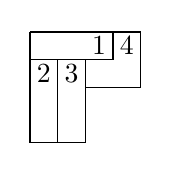
\begin{tikzpicture}[baseline=(current bounding box.center)]
\begin{scope}[yscale=-1]
 \begin{scope}[xshift=0em,yshift=0em]
\pic{hTrio}; 
\end{scope}
\begin{scope}[xshift=0em,yshift=1em]
\pic{iTrio}; 
\end{scope}
\begin{scope}[xshift=1em,yshift=1em]
\pic{iTrio}; 
\end{scope}
\begin{scope}[xshift=2em]
\pic{jTrio}; 
\end{scope}
\begin{scope}[xshift=-0.5em,yshift=-0.5em]
\node[x=1em,y=1em] at (3,1) {1};
\node[x=1em,y=1em] at (1,2) {2};
\node[x=1em,y=1em] at (4,1) {4};
\node[x=1em,y=1em] at (2,2) {3};
\end{scope}
\end{scope}
\end{tikzpicture}


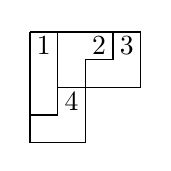
\begin{tikzpicture}[baseline=(current bounding box.center)]
\begin{scope}[yscale=-1]
 \begin{scope}[xshift=0em,yshift=0em]
\pic{iTrio}; 
\end{scope}
\begin{scope}[xshift=1em,yshift=0em]
\pic{tTrio}; 
\end{scope}
\begin{scope}[xshift=0em,yshift=2em]
\pic{jTrio};
\end{scope}
\begin{scope}[xshift=2em]
\pic{jTrio};
\end{scope}
\begin{scope}[xshift=-0.5em,yshift=-0.5em]
\node[x=1em,y=1em] at (3,1) {2};
\node[x=1em,y=1em] at (1,1) {1};
\node[x=1em,y=1em] at (4,1) {3};
\node[x=1em,y=1em] at (2,3) {4};
\end{scope}
\end{scope}
\end{tikzpicture}


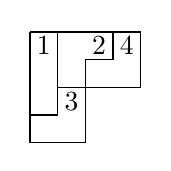
\begin{tikzpicture}[baseline=(current bounding box.center)]
\begin{scope}[yscale=-1]
 \begin{scope}[xshift=0em,yshift=0em]
\pic{iTrio}; 
\end{scope}
\begin{scope}[xshift=1em,yshift=0em]
\pic{tTrio}; 
\end{scope}
\begin{scope}[xshift=0em,yshift=2em]
\pic{jTrio};
\end{scope}
\begin{scope}[xshift=2em]
\pic{jTrio};
\end{scope}
\begin{scope}[xshift=-0.5em,yshift=-0.5em]
\node[x=1em,y=1em] at (3,1) {2};
\node[x=1em,y=1em] at (1,1) {1};
\node[x=1em,y=1em] at (4,1) {4};
\node[x=1em,y=1em] at (2,3) {3};
\end{scope}
\end{scope}
\end{tikzpicture}


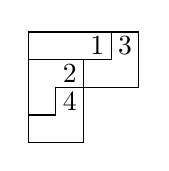
\begin{tikzpicture}[baseline=(current bounding box.center)]
\begin{scope}[yscale=-1]
 \begin{scope}[xshift=0em,yshift=0em]
\pic{hTrio}; 
\end{scope}
\begin{scope}[xshift=0em,yshift=1em]
\pic{tTrio}; 
\end{scope}
\begin{scope}[xshift=0em,yshift=2em]
\pic{jTrio}; 
\end{scope}
\begin{scope}[xshift=2em]
\pic{jTrio}; 
\end{scope}
\begin{scope}[xshift=-0.5em,yshift=-0.5em]
\node[x=1em,y=1em] at (3,1) {1};
\node[x=1em,y=1em] at (2,2) {2};
\node[x=1em,y=1em] at (4,1) {3};
\node[x=1em,y=1em] at (2,3) {4};
\end{scope}
\end{scope}
\end{tikzpicture}


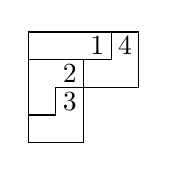
\begin{tikzpicture}[baseline=(current bounding box.center)]
\begin{scope}[yscale=-1]
 \begin{scope}[xshift=0em,yshift=0em]
\pic{hTrio}; 
\end{scope}
\begin{scope}[xshift=0em,yshift=1em]
\pic{tTrio}; 
\end{scope}
\begin{scope}[xshift=0em,yshift=2em]
\pic{jTrio}; 
\end{scope}
\begin{scope}[xshift=2em]
\pic{jTrio}; 
\end{scope}
\begin{scope}[xshift=-0.5em,yshift=-0.5em]
\node[x=1em,y=1em] at (3,1) {1};
\node[x=1em,y=1em] at (2,2) {2};
\node[x=1em,y=1em] at (4,1) {4};
\node[x=1em,y=1em] at (2,3) {3};
\end{scope}
\end{scope}
\end{tikzpicture}

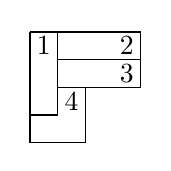
\begin{tikzpicture}[baseline=(current bounding box.center)]
\begin{scope}[yscale=-1]
 \begin{scope}[xshift=0em,yshift=0em]
\pic{iTrio}; 
\end{scope}
\begin{scope}[xshift=1em,yshift=0em]
\pic{hTrio}; 
\end{scope}
\begin{scope}[xshift=1em,yshift=1em]
\pic{hTrio}; 
\end{scope}
\begin{scope}[yshift=2em]
\pic{jTrio};
\end{scope}
\begin{scope}[xshift=-0.5em,yshift=-0.5em]
\node[x=1em,y=1em] at (4,1) {2};
\node[x=1em,y=1em] at (1,1) {1};
\node[x=1em,y=1em] at (4,2) {3};
\node[x=1em,y=1em] at (2,3) {4};
\end{scope}
\end{scope}
\end{tikzpicture}


\end{document}

